\documentclass[a4paper,titlepage,11pt]{article}

\usepackage[top=2.54cm, bottom=2.54cm, left=2.54cm, right=2.54cm]{geometry}
\usepackage[utf8x]{inputenc}
\usepackage{hyperref}
\usepackage{graphicx}
\usepackage{fancyhdr}
\usepackage{lastpage}

\pagestyle{fancy}
\fancyhf{}
\renewcommand{\headrulewidth}{0pt}
\cfoot{ \thepage \hspace{1pt} of \pageref{LastPage} }

\begin{document}

\begin{titlepage}
  \begin{center}
    {\scshape \huge Truthful Emergencies \par}
    \vspace{1cm}

    {\scshape \LARGE Report \par}
    \vspace{1.5cm}

    {\scshape \Large Network and Computer Security \par}
    \vspace{0.5cm}

    {\Large Alameda \par}
    \vfill

    {\itshape \Large Group 11 \par}
    \vfill

    \begin{tabular}{l l l}
      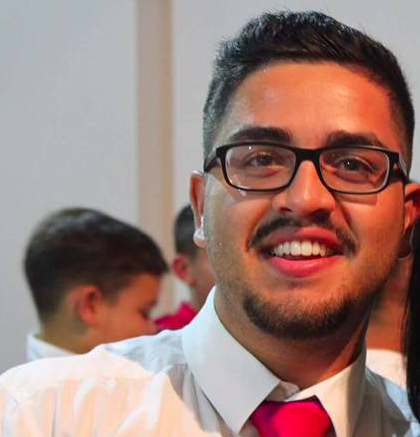
\includegraphics[width=20mm, height=20mm]{img/miguel.png} & Miguel Pinto & 79060\\
      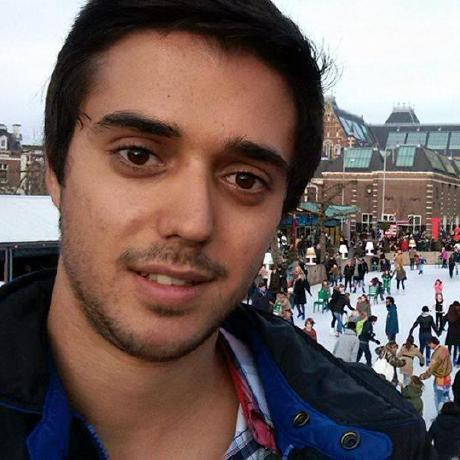
\includegraphics[width=20mm, height=20mm]{img/bernardo.jpeg} & Bernardo Casaleiro & 87827\\
      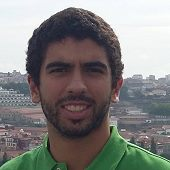
\includegraphics[width=20mm, height=20mm]{img/joao.jpeg} & João Godinho & 87830\\
    \end{tabular}
    \vfill

    {\large \today\par}
  \end{center}
\end{titlepage}

\section{Problem}
First response emergency systems are a limited resource. Their usage makes a difference in life-or-death situations!
Requesting an ambulance is a serious matter.
It should be simple, secure, fast and first of all always available.
For that the Dispatch Center must be fault tolerant.

It should separate the real requests from the false ones and provide a response accordingly.
Improper usage must be detected to avoid misallocation of resources while real requests should
trigger an appropriate response.

\section{Requirements}

\subsection{Application Requirements}
\begin{enumerate}
  \item Send an emergency request.
  \item Inform the estimated time for the user's request to be answered.
\end{enumerate}

\subsection{Server Requirements}
\begin{enumerate}
  \item Receive a request
  \item Insert a request in a queue depending on the user rating.
  \item Log the requests.
  \item Send the expected response time.
  \item Send the confirmation that an ambulance is on route.
  \item Rate the user accordingly at the end of the request.
  \item Temporarily block a user for abusive usage.
\end{enumerate}

\subsection{Security Requirements}
\begin{enumerate}
  \item Non-repudiation.
  \item Fault tolerance to DoS.
  \item Filter, responsible for filtering the requests.
  \item Auditing mechanisms.
  \item Secure channel between user and Dispatch Central.
\end{enumerate}

\section{Implemented solution}

\begin{figure}[h]
    \centering
    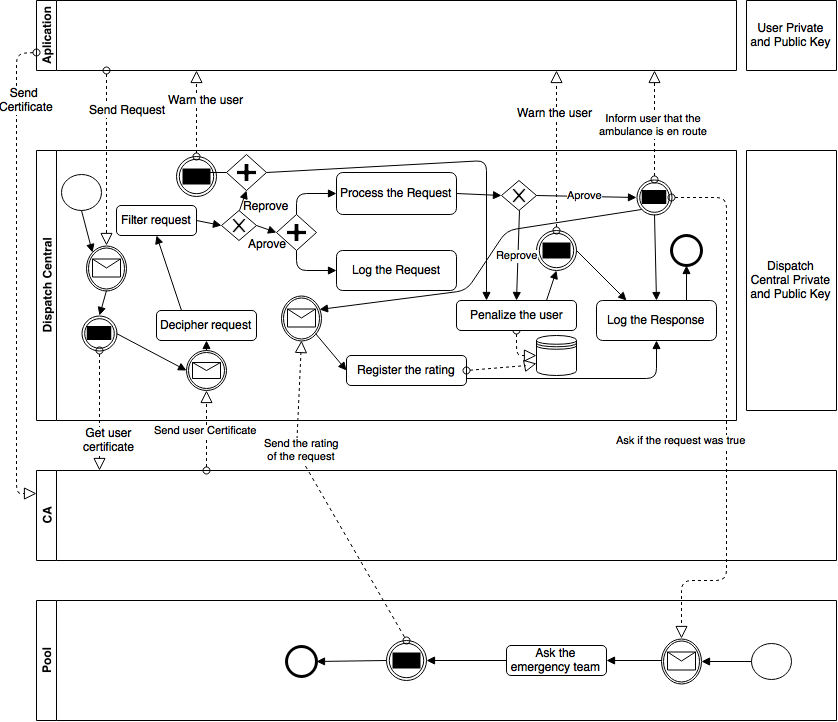
\includegraphics[scale=0.50]{img/advanced-solution.png}
\end{figure}

% TODO: Non-Repudiation
% TODO: Fault tolerance to DoS.
% TODO: Auditing mechanisms
% TODO: Secure channel

\section{Results}

\section{Evaluation}

\section{Conclusion}

\section{References}

\subsection{Tool References}
\begin{description}
  \item [PostgreSQL] \href{https://www.postgresql.org}{Database to save the users.}
  \item [javax.net.ssl.SSLServerSocket] \href{https://docs.oracle.com/javase/7/docs/api/java/net/Socket.html}{Establish a secure connection between the server and the application.}
  \item [PostgreSQL JDBC] \href{https://jdbc.postgresql.org}{Driver to use PostgreSQL with Java.}
\end{description}

\end{document}
